%-------------------------------------------------------------------------------
% LATEX TEMPLATE ARTIKEL
%-------------------------------------------------------------------------------
% Dit template is voor gebruik door studenten van de de bacheloropleiding 
% Informatica van de Universiteit van Amsterdam.
% Voor informatie over schrijfvaardigheden, zie 
%                               https://practicumav.nl/schrijven/index.html
%
%-------------------------------------------------------------------------------
%	PACKAGES EN DOCUMENT CONFIGURATIE
%-------------------------------------------------------------------------------

\documentclass{uva-inf-article}
\usepackage[english]{babel}
\usepackage{colortbl}
\usepackage{graphicx}
\usepackage{listings}
\usepackage{booktabs}
\usepackage{subcaption}
\usepackage{lipsum}
\usepackage{amsmath}
\usepackage{apacite}
% \usepackage[style=authoryear-comp, style=apalike]{biblatex}
% \addbibresource{references.bib}

\captionsetup[figure]{labelfont=bf,width=0.8\linewidth}
\captionsetup[table]{labelfont=bf,width=0.8\linewidth}

%-------------------------------------------------------------------------------
%	GEGEVENS VOOR IN DE TITEL, HEADER EN FOOTER
%-------------------------------------------------------------------------------

\newcommand{\sk}[1]{\textcolor{blue}{#1}}
\newcommand{\ad}[1]{\textcolor{red}{#1}}

% Geef je artikel een logische titel die de inhoud dekt.
\title{Title}

% Vul de naam van de opdracht in zoals gegeven door de docent en het type 
% opdracht, bijvoorbeeld 'technisch rapport' of 'essay'.
\assignment{Assignment III: Simulated Annealing}
\assignmenttype{Coding exercise}

% Vul de volledige namen van alle auteurs in en de corresponderende UvAnetID's.
\authors{Annemijn Dijkhuis; Sam Kuilboer}
\uvanetids{11149272; 12442690}

% Vul de naam van je tutor, begeleider (mentor), of docent / vakcoördinator in.
% Vermeld in ieder geval de naam van diegene die het artikel nakijkt!
\tutor{}
\mentor{}
\docent{}

% Vul hier de naam van je tutorgroep, werkgroep, of practicumgroep in.
\group{Group 32}

% Vul de naam van de cursus in en de cursuscode, te vinden op o.a. DataNose.
\course{Stochastic Simulation}
\courseid{}

% Dit is de datum die op het document komt te staan. Standaard is dat vandaag.
\date{\today}

%-------------------------------------------------------------------------------
%	VOORPAGINA 
%-------------------------------------------------------------------------------

\begin{document}
\maketitle

%-------------------------------------------------------------------------------
%	INHOUDSOPGAVE EN ABSTRACT
%-------------------------------------------------------------------------------
% Niet toevoegen bij een kort artikel, zeg minder dan 10 pagina's!

%TC:ignore
%\tableofcontents
%\begin{abstract}
%\end{abstract}
%TC:endignore

%-------------------------------------------------------------------------------
%	INHOUD
%-------------------------------------------------------------------------------
% Hanteer bij benadering IMRAD: Introduction, Method, Results, Discussion.
\begin{abstract}
 \ad{abstract}
\end{abstract}

\newpage

\section{Introduction}



% \begin{figure}
%     \centering
%     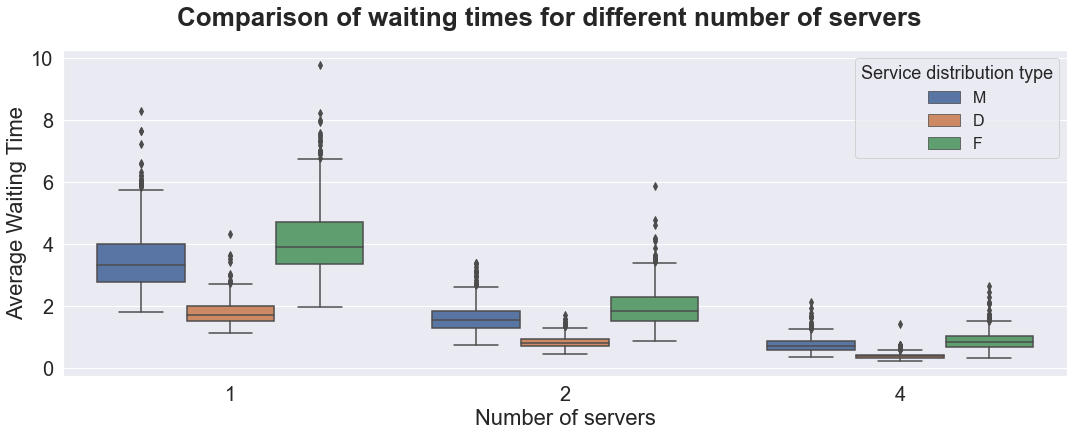
\includegraphics[width=\linewidth]{figures/boxplotDistributions.png}
%     \caption{Boxplot representing the average waiting times for the multiple server configurations and service time distributions. The increment of servers reduces the waiting time as does the implementation of a deterministic service time distribution in comparison to the exponential distribution. The fat-tail distribution extended the on average waiting time ($\mu=2.5$ , $\rho=0.9$, $\lambda_1 = 2.25$, $\lambda_2 = 4.50$, $\lambda_4 = 9.00$, $N=5000$, $s=500$).}
%     \label{fig:boxplotDistributions}
% \end{figure}


\section{Discussion}

%-------------------------------------------------------------------------------
%	REFERENTIES
%-------------------------------------------------------------------------------
\bibliographystyle{apacite}
% \printbibliography
\bibliography{references}
%-------------------------------------------------------------------------------
%	BIJLAGEN 
%-------------------------------------------------------------------------------

%TC:ignore
%TC:endignore

%-------------------------------------------------------------------------------
\end{document}

